\documentclass[10pt]{article}
\usepackage[ngerman]{babel}
\usepackage{graphicx}
\usepackage{hyperref}
\usepackage{cleveref}
\usepackage[%
  backend=biber,
  style=alphabetic,
  sorting=ynt]{biblatex}
\addbibresource{bib.bib}
\author{Maximilian Heim}
\title{Identitäts und Berechtigungsmanagement}
\begin{document}
\maketitle
\newpage
\tableofcontents
\newpage
\section{Einleitung}
\subsection{Aufgabenstellung}
\subsection{Forschungsfragen}
Diese Seminararbeit soll dem Leser eine gute Grundlage dafür geben, sich mit dem Thema Identitäts- und Berechtigungsmanagement auseinanderzusetzen.
\begin{itemize}
  \item In Kapitel ~\cref{sec:grundlagen} werden die Begriffe Identität, Berechtigung und Identitäts- und Berechtigungsmanagement eingeführt um eine Grundlage für die weitere Arbeit zu haben.
  \item In Kapitel ~\cref{sec:existing} werden die existierenden Methoden, Standards, Technologien und Tools zusammenfassend beschreiben.
  \item In Kapitel ~\cref{sec:betrieb} wird der Kontext von IAM im betrieblichen Kontext beschrieben.
\end{itemize}
\section{Grundlagen}
\label{sec:grundlagen}
\subsection{Einordnung}
\subsection{Identität}
Um den Begriff Identitätsmanagement zu definieren sollte zuerst der Begriff der Identität definiert werden. In der Philosophie wird Identität über die Ununterscheidbarkeit von Dingen definiert. Nach dem Identitätsprinzip sind zwei Dinge genau dann identisch wenn sich zwischen ihnen keine Unterschiede finden lassen. Hierbei geht es um die Fragestellung "wer bist du?". Im Kontext der IT wird dies durch Authentifizierungsverfahren umgesetzt. In der IT haben sich eine Vielzahl an Authentifizierungsverfahren durchgesetzt. Für einen kurzen Überblick sind einige Authentifizierungsverfahren im folgenden aufgelistet.
\begin{itemize}
  \item Passwörter und Pins sind die wohl bekanntesten Arten der Authentifizierung. Jedoch ist es auch eine der unsichersten Arten da diese gerne mehrfach verwendet werden oder geknackt werden können
  \item Tokens sind eine andere Art der Authentifizierung die auf Besitz und Wissen basieren und daher sicherer sind wie rein wissensbasierte Verfahren. Hierbei wird ein Gerät verwendet welches nach Entsperrung mittels Pin/Passwort ein Einmalpasswort ausgibt oder automatisch die Authentifizierung freigibt
  \item Eine weiteres Beispiel für Authentifizierung ist die Biometrie. Hierbei werden z.B. der Fingerabdruck, die Retina oder die Stimme einer Person verwendet um diese zu identifizieren
\end{itemize}
~\cite{tsolkas2017}
\subsection{Identitätsmanagement}
Identitätsmanagement beschreibt die Verwaltung von digitalen Identitäten. Hierbei werden Prozesse für die Provisonierung, Änderung und Deprovisionierung von digitalen Identitäten definiert und umgesetzt.~\cite{sharma2016identity}
\subsection{Berechtigung}
Berechtigungen oder auch Zugriffsberechtigungen beschreiben welche Identitäten auf welche Ressourcen zugreifen darf. Dieser Prozess findet nach der Authentifizierung statt. Hierbei geht es um die Fragestellung "was darf er/sie/es?". Die Kontrolle der Berechtigungen basierend auf einer Identität wird Zugriffskontrolle oder auch Autorisierung genannt.~\cite{tsolkas2017}
\subsection{Berechtigungsmanagement}
Berechtigungsmanagement ist verantwortlich für die Festlegung welche Nutzer/Entitäten auf welche Ressourcen Zugriff haben. Beispiele hierfür sind der Zugriff auf eine Datenbank, der Zugriff auf Dokumente oder der Konfiguration von Systemen. Das Ziel ist hierbei ist das Least-Privilege-Prinzip (PoLP) umzusetzen. Das Berechtigungsmanagement besteht aus verschiedenen Aspekten. So z.B. der Provisionierung von Rechten, der Compliance mit Standards und der konkreten technischen Umsetzung der Authorisierung.
\begin{figure}
  \centering
  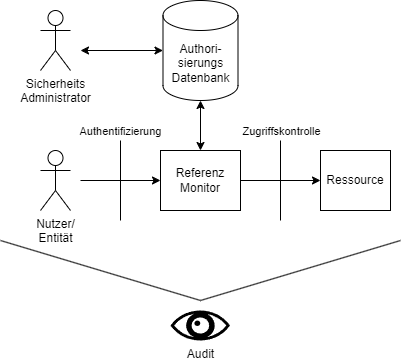
\includegraphics[width=0.7\textwidth]{assets/accessmanagement.png}
  \label{fig:accesscontrol}
  \caption{Abstrakte Einordnung der Zugriffskontrolle [Basiert auf "Access Control: Principles and Practice von Ravi S. Sandhu and Pierangela Samarati"]}
\end{figure}
\subsection{Erkenntnisse im Kontext von IT-GRC}
Das Identitäts und Berechtigungsmanagement ist eine zentrale Disziplin im Kontext der IT-GRC. Die sorgfältige Umsetzung von Identitäts- und Berechtigungsmanagement hilft dabei IT-Sicherheits-Risiken zu minimieren und die Compliance von Standards zu gewährleisten.
\section{Methoden, Technologien und Tools}
\label{sec:existing}
\subsection{Betriebliche Motivation}
\subsection{Standards}
\paragraph{BSI}
Das Bundesamt für Sicherheit der Informationstechnik (BSI) definiert mit BSI-Standard 200-3 einen Leitfaden zur Risikobewertung. In BSI-Standard 200-1 werden Sicherheitsmaßnahmen definiert die zur Behandlung der Risiken geeignet sind. In Bezug auf den BSI-Standard definiert das IT-Grundschutz-Kompendium des BSI's Prozessbausteine zur Umsetzung des ISMS. Hier wird im Prozessbaustein "ORP.4 Identitäts- und Berechtigungsmanagent" auf verschiedene Anforderungen für die Umsetzung von IAM eingegangen. Kapitel 3.1 definiert Basis-Anforderungen welche umgesetzt werden müssen. Kapitel 3.2 definiert Standard-Anforderungen welche umgesetzt werden sollten. Kapitel 3.3 definiert Anforderungen welche bei erhöhtem Schutzbedarf umgesetzt werden sollten. Das IT-Grundschuztz-Kompendium definiert zusätzlich zu ORP.4 System-Bausteine wie SYS.1.3 und APP.2.1. Diese enthalten konkrete Maßnahmen zur Umsetzung des IAM für System-Komponenten wie Betriebssysteme und Verzeichnisdienste.
\paragraph{ISO 27001 Annex A.9}
ISO 27001 definiert mit Anhang A.9 die Zugangssteuerung.
\paragraph{SO/IEC 29146}
\paragraph{NIST 800-53A}
Das National Institute of Standards and Technology (NIST) publizierte die "NIST Special Publication 800-53A - Assessing Security and Privacy Controls in Information Systems and Organizations". Dieses Dokument stellt Prozesse und Methoden für die Bewertung von Sicherheits- und Datenschutzmaßnahmen vor. Im Kapitel "Security and Privacy Assessment Procedures" wird im Unterkapitel 4.1 "Access Control Family (AC)" auf Zugangskontrolle und im Unterkapitel 4.7 "Identification and Authentication Family (IA)" auf Identifizierung und Authentifizierung eingegangen.
\subsection{Methoden und Prozesse}
\subsection{Technologien und Tools}
IAM Tools ersetzen nicht die Einhaltung von Standards und die sorgfältige Planung von IAM Prozessen. Sie sind jedoch hilfreiche Werkzeuge zur technischen Umsetzung von IAM.
\paragraph{SAML}
SAML ist ein weit verbreiteter Standard zur Umsetzung von Sicherheits Assertationen. Mit SAML wird ein XML Format definiert welches zur Authentifizierung und Authorisierung von Nutzern verwendet werden kann. Im Kontext von SAML werden verschiedene Begrifflichkeiten definiert.
\begin{itemize}
  \item Assertation - Eine Assertation über die Charakteristiken und Attribute eines Subjekts. So z.B. die Zugehörigkeit zu einer Gruppe oder der Besitz eines Attributs.
  \item Identity Provider (IdP) - Der Server der für die eigentliche Bearbeitung der Assertation zuständig ist. Er erhält die Anfrage und leitet die Antwort an den Service Provider weiter.
  \item Service Provider (SP) - Das Ziel der Authentifizierung/Authorisierung, dieser stellt eine Ressource/Service zur Verfügung.
\end{itemize}
~\cite{hughes2005security}
\paragraph{OAuth}

\paragraph{IBM Security Verify}
Das Unternehmen IBM bietet mit dem Produkt "IBM Security Verify" eine Cloud basierte Lösung zum Identitäts- und Berechtigungsmanagement. Dieses Produkt bietet umfangreiche Funktionalitäten wie SSO, MFA, KI gestütze Risikobewertung von Zugriffen und Identitätsanalyse, d.h. die Analyse von Identitäten und Berechtigungen zum Zweck der Identifizierung von Abweichungen.
\paragraph{Microsoft Active Directory}
\paragraph{Microsoft Entra ID}
Das Unternehmen Microsoft bietet mit dem Produkt "Microsoft Entra ID" eine Cloud basierte Lösung zum Identitäts- und Berechtigungsmanagement von Microsoft und Drittpartei Dienste. Dieses Produkt bietet viele Vorteile. So z.B. eine Multi-Faktor-Authentifizierung mittels Microsoft Authenticator.
\paragraph{SAP Cloud Identity Access Governance}
Das Unternehmen SAP bietet mit dem Produkt "SAP Cloud Identity Access Governenace" eine Cloud basierte Lösung zum Identitäts- und Berechtigungsmanagement. SAP selbst schreibt dem Produkt eine intuitive Bedienung, hohe Anpassbarkeit und skalierbare Funktionen zu.
\paragraph{Okta Inc.}
Das Unternehmen Okta Inc. ist ein in den USA ansässiges Unternehmen welches sich auf IAM spezialisiert hat. Mit rund 6000 Mitarbeitern und mehr als einer Milliarde US-Dollar an Umsatz ist es ein führender Hersteller von IAM Produkten. Vom Unternehmen werden 2 Produkte angeboten. Customer Identity Cloud und Workforce Identity Cloud. Customer Identity Cloud ist eine Lösung zum Customer Identity Management, d.h. es ermöglicht die sichere Verwaltung und Authentifizierung von Kunden-Identitäten. Workforce Identity Cloud ist eine Lösung zum Unternehmensinternen Identitätsmanagement.
\subsection{Erkenntnisse im Kontext von IT-GRC}
\section{Betriebliches Identitäts- und Berechtigungsmanagement}
\label{sec:betrieb}
\subsection{Überblick}
\subsection{Organisatorische Aspekte}
Das Identitäts- und Berechtigungsmanagement fällt unter die Domäne der Informations- und IT-Sicherheit. Auf der Führungsebene ist im Unternehmen der Chief Information Security Officer (CISO) für die Umsetzung des Informationssicherheitsmanagementsystems (CISO) verantwortlich. Daher trägt der CISO in diesem Kontext eine Führende Rolle. Im Fall von umfangreichen Anforderungen an das System kann die Umsetzung des IAM ein ganzes Team benötigen.
\subsection{Technische Aspekte}
\subsection{Wirtschaftliche Aspekte}
\subsection{Erkenntnisse im Kontext von IT-GRC}
\section{Fazit}
\subsection{Zusammenfassung}
\subsection{Beantwortung der Forschungsfragen}
\section{Eidesstattliche Versicherung}
\newpage
\section{Literaturverzeichnis}
\printbibliography
\newpage
\section{Quellenverzeichnis}
\newpage
\listoffigures
\end{document}